\chapter{Additional material for the FIR filter}
This chapter provides the definitions of 5 common windows, the derivation of the ideal impulse response, and the amplitude responses of the windows used in the filter theory and the implementation of the filter in chapters \ref{ch8} and \ref{ch10}, respectively.

\input{sections/appE/appEwindows_table.tex}
\clearpage

\section{Derivation of ideal impulse response}\label{appC}
In order to derive the ideal impulse response for the bandpass filter described in chapter \ref{ch10} the ideal frequency response is defined as follows based on figure \ref{fig:spec_Hd}:
%\begin{align*}
% H_d(\text{e}^{j\omega}) = \begin{cases}
% 0, \ \ \ & |\omega| \leq \omega_{c_1} \\
%  \text{e}^{-j\omega\frac{M}{2}}, \ \ \ & \omega_{c_1} \leq | \omega | \leq \omega_{c_2} \\
%  0, \ \ \ & \omega_{c_2} \leq |\omega| \leq \pi 
%\end{cases}
%\end{align*}

\begin{align*}
H_d(\text{e}^{j\omega}) = \begin{cases}
\text{e}^{-j\omega\frac{M}{2}}, \quad &\begin{cases}
-\omega_{c_2} \leq \omega \leq -\omega_{c_1} \\
\omega_{c_1} \leq \omega \leq \omega_{c_2}
\end{cases} \\
0, \quad &Otherwise
\end{cases}
\end{align*}

From this the ideal impulse response is determined by the inverse Fourier transform described in definition \ref{def:InverseFourier_trans}:
\begin{align*}
h_d[n] &= \dfrac{1}{2\pi} \int_{-\pi}^\pi H_d(\text{e}^{j\omega}) \text{e}^{j\omega n} d\omega = \dfrac{1}{2\pi} \left(  \int_{-\omega_{c_2}}^{-\omega_{c_1}} \text{e}^{-j\omega \frac{M}{2}} \cdot \text{e}^{j \omega n} d\omega + \int_{\omega_{c_1}}^{\omega_{c_2}} \text{e}^{-j\omega \frac{M}{2}} \cdot \text{e}^{j \omega n} d\omega \right) \\
&= \frac{1}{2\pi} \left( \int_{-\omega_{c_2}}^{-\omega_{c_1}} \text{e}^{j\omega \left(n - \frac{M}{2} \right) } d\omega + \int_{\omega_{c_1}}^{\omega_{c_2}} \text{e}^{j\omega \left(n- \frac{M}{2} \right)} d\omega \right).
\end{align*}

According to Euler's formula $\text{e}^{j\omega t} = \cos(\omega t) + j\sin(\omega t)$. For the first integral above it follows that
\begin{align*}
\int_{-\omega_{c_2}}^{-\omega_{c_1}} \text{e}^{j\omega \left(n- \frac{M}{2} \right)} d\omega &= \int_{-\omega_{c_2}}^{-\omega_{c_1}} \cos \left( \omega \left(n-\dfrac{M}{2}\right)\right) + j \sin \left( \omega \left(n-\dfrac{M}{2}\right) \right) d\omega \\
&= \left[ \sin\left(\omega \left(n-\dfrac{M}{2}\right)\right) \right]_{\omega=-\omega_{c_2}}^{-\omega_{c_1}} \cdot \dfrac{1}{n - \frac{M}{2}}
\end{align*}

since the integral of the second term evaluates to 0. Since $\sin(-\omega\cdot t) = - \sin(\omega \cdot t)$ the impulse response may be written as
\begin{align*}
h_d[n] &= \dfrac{1}{2\pi} \left( \dfrac{1}{n - \frac{M}{2}} \left( \sin \left( - \omega_{c_1} \left( n - \frac{M}{2} \right) \right) - \sin \left( - \omega_{c_2} \left( n - \frac{M}{2} \right) \right) + \sin \left( \omega_{c_2} \left( n - \frac{M}{2} \right) \right) - \sin \left( \omega_{c_1} \left( n - \frac{M}{2} \right) \right) \right) \right) \\
&= \dfrac{1}{2\pi} \left( \dfrac{1}{n - \frac{M}{2}} \left( - \sin \left( \omega_{c_1} \left( n - \frac{M}{2} \right) \right) + \sin \left( \omega_{c_2} \left( n - \frac{M}{2} \right) \right) + \sin \left( \omega_{c_2} \left( n - \frac{M}{2} \right) \right) - \sin \left( \omega_{c_1} \left( n - \frac{M}{2} \right) \right) \right) \right) \\
&= \dfrac{1}{2\pi} \left( \dfrac{2}{n - \frac{M}{2}} \left( - \sin \left( \omega_{c_1} \left( n - \frac{M}{2} \right) \right) + \sin \left( \omega_{c_2} \left( n - \frac{M}{2} \right) \right) \right) \right) \\
&= \dfrac{1}{\pi \left( n - \frac{M}{2}\right)} \left( \sin\left( \omega_{c_2} \left( n - \frac{M}{2} \right) \right) - \sin \left( \omega_{c_1} \left( n - \frac{M}{2} \right) \right) \right).
\end{align*}

This is only true for $n \neq \frac{M}{2}$, and $h_d[M/2]$ must be defined separately. In order to do so l'Hôspital's rule$^[$\footnote{A more detailed version of l'Hôpital's rule may be found at \url{http://tutorial.math.lamar.edu/Classes/CalcI/LHospitalsRule.aspx}.}$^]$, which says that $\lim \frac{f(x)}{g(x)} = \lim \frac{f'(x)}{g'(x)}$, is used. Thus:
\begin{align*}
h_d[M/2] &= \dfrac{d}{dn} \left[ \dfrac{1}{\pi \left( n - \frac{M}{2}\right)} \left( \sin\left( \omega_{c_2} \left( n - \frac{M}{2} \right) \right) - \sin \left( \omega_{c_1} \left( n - \frac{M}{2} \right) \right) \right) \right]_{n = \frac{M}{2}} \\
&= \dfrac{1}{\pi} (\cos (\omega_{c_2} \cdot 0) \omega_{c_2} - \cos (\omega_{c_1} \cdot 0) \omega_{c_1}) = \dfrac{1}{\pi} ( \omega_{c_2} - \omega_{c_1})
\end{align*}

Collectively, the ideal impulse response is:
\begin{align*}
h_d[n] = \begin{cases}
\dfrac{1}{\pi \left( n - \frac{M}{2}\right)} \left( \sin\left( \omega_{c_2} \left( n - \frac{M}{2} \right) \right) - \sin \left( \omega_{c_1} \left( n - \frac{M}{2} \right) \right) \right), \quad &n \neq \dfrac{M}{2} \\
\dfrac{1}{\pi} ( \omega_{c_2} - \omega_{c_1}), \quad &n = \dfrac{M}{2}
\end{cases}.
\end{align*}

\clearpage
\chapter{Amplitude responses of windows} \label{appD}
The figures below show the amplitude responses in dB of the different windows considered for the STFT in section \ref{sec:STFT_variation}.

\begin{figure}[H]
\centering
\begin{subfigure}{0.49\textwidth}
\centering
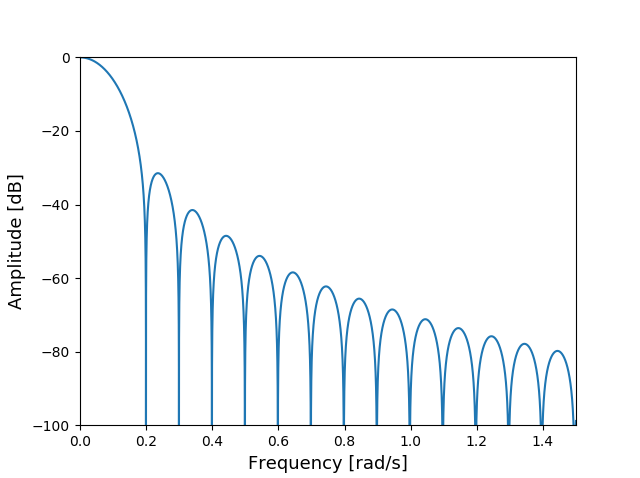
\includegraphics[width=\textwidth]{figures/dbplots/stft_bilag/64/hann.png}
\caption{Hann}
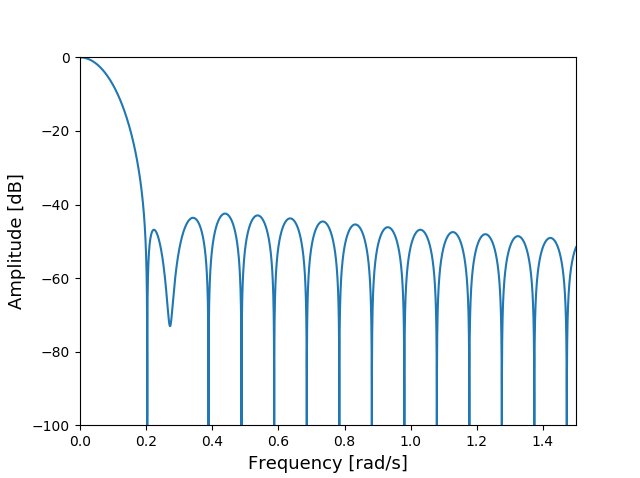
\includegraphics[width=\textwidth]{figures/dbplots/stft_bilag/64/hamming.png}
\caption{Hamming}
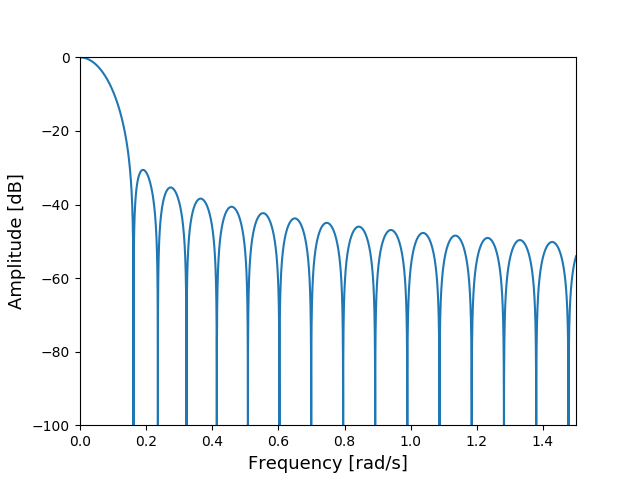
\includegraphics[width=\textwidth]{figures/dbplots/stft_bilag/64/kaiser4.png}
\caption{Kaiser, $\beta=4$}
\end{subfigure}
\centering
\begin{subfigure}{0.49\textwidth}
\centering
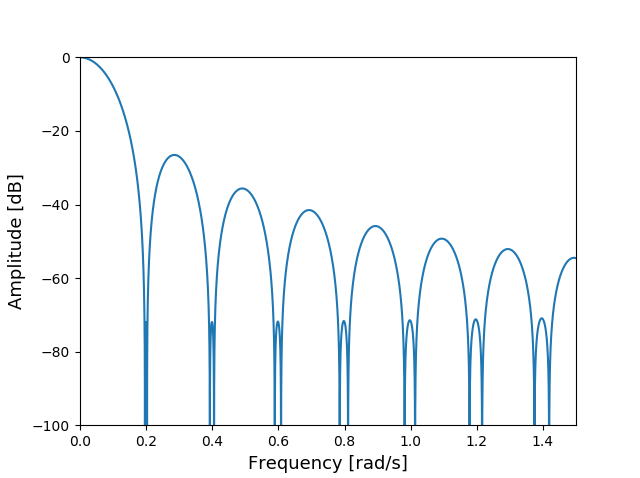
\includegraphics[width=\textwidth]{figures/dbplots/stft_bilag/64/bartlett.png}
\caption{Bartlett}
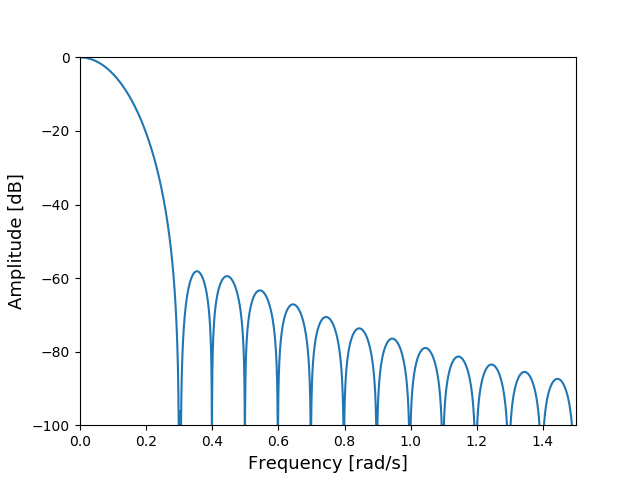
\includegraphics[width=\textwidth]{figures/dbplots/stft_bilag/64/blackman.png}
\caption{Blackman}
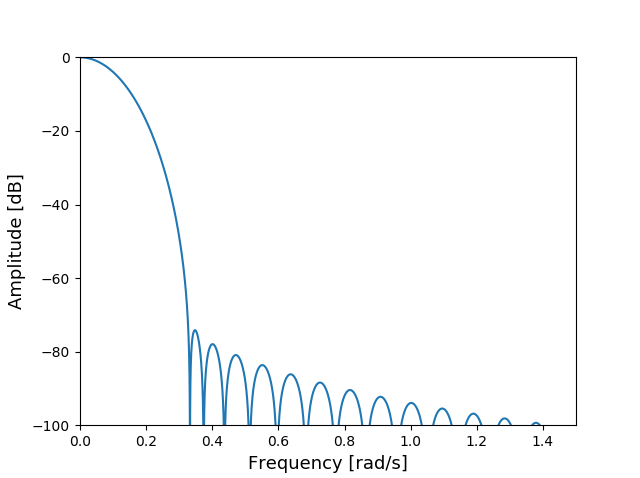
\includegraphics[width=\textwidth]{figures/dbplots/stft_bilag/64/kaiser10.png}
\caption{Kaiser, $\beta=10$}
\end{subfigure}

\caption{Amplitude response of window functions of order $M=64$}
\label{fig:db_plots_64}
\end{figure}

\begin{figure}[H]
\centering

\begin{subfigure}{0.49\textwidth}
\centering
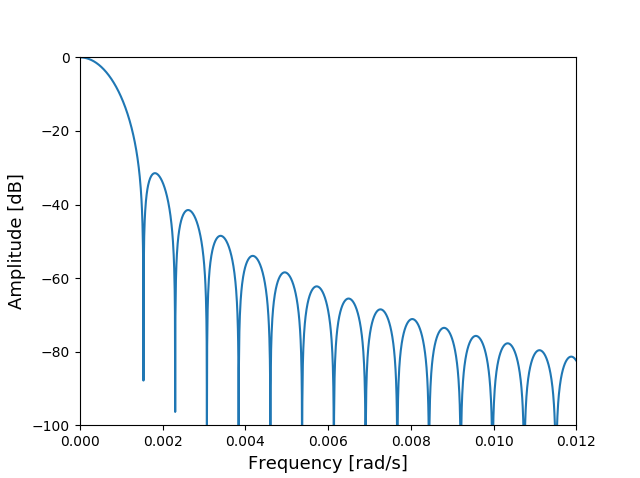
\includegraphics[width=\textwidth]{figures/dbplots/stft_bilag/8192/hann.png}
\caption{Hann}
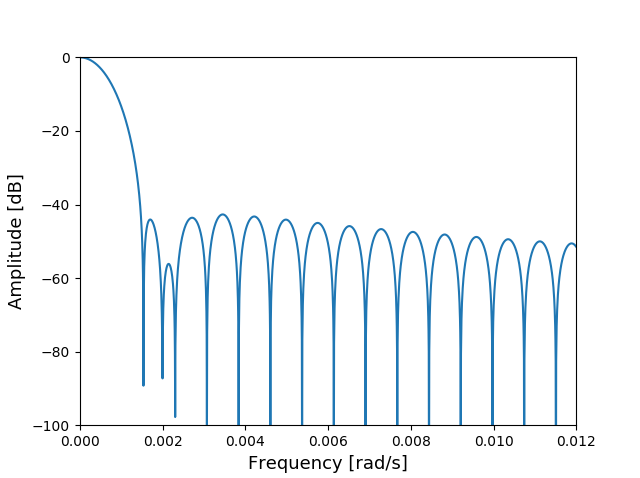
\includegraphics[width=\textwidth]{figures/dbplots/stft_bilag/8192/hamming.png}
\caption{Hamming}
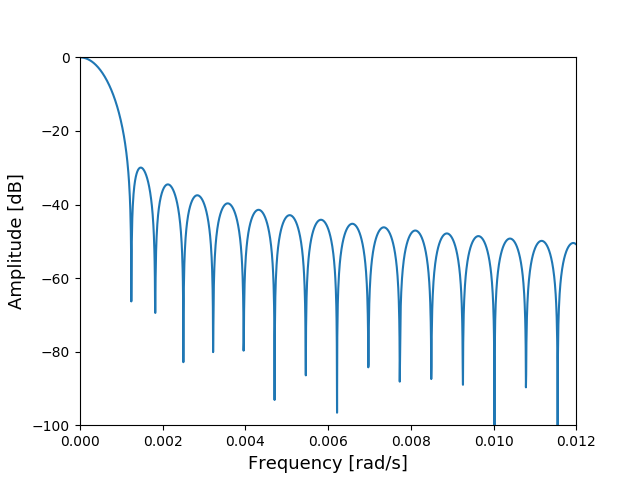
\includegraphics[width=\textwidth]{figures/dbplots/stft_bilag/8192/kaiser4.png}
\caption{Kaiser, $\beta=4$}
\end{subfigure}
\centering
\begin{subfigure}{0.49\textwidth}
\centering
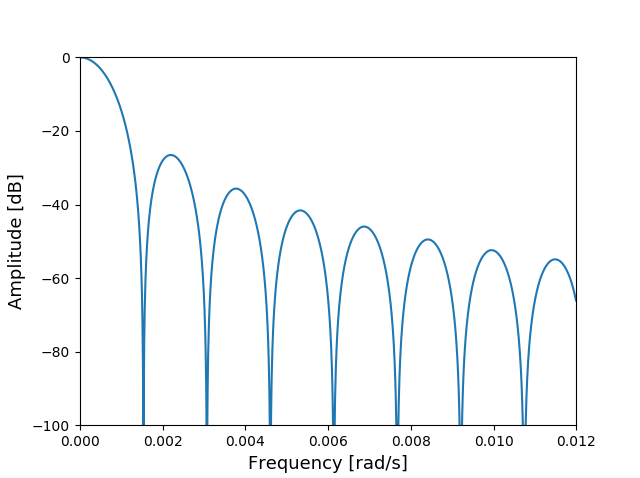
\includegraphics[width=\textwidth]{figures/dbplots/stft_bilag/8192/bartlett.png}
\caption{Bartlett}
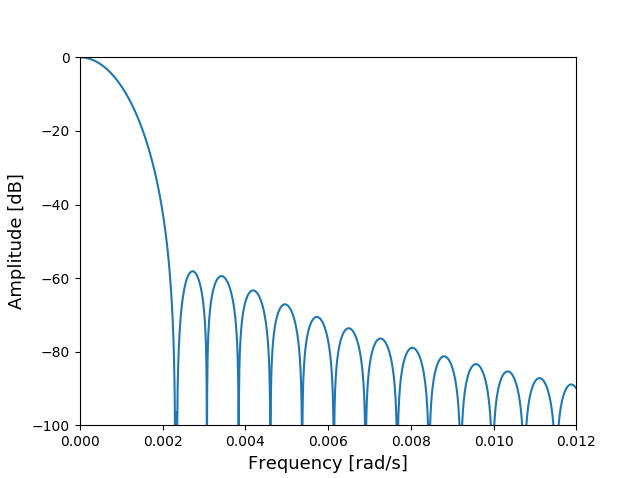
\includegraphics[width=\textwidth]{figures/dbplots/stft_bilag/8192/blackman.png}
\caption{Blackman}
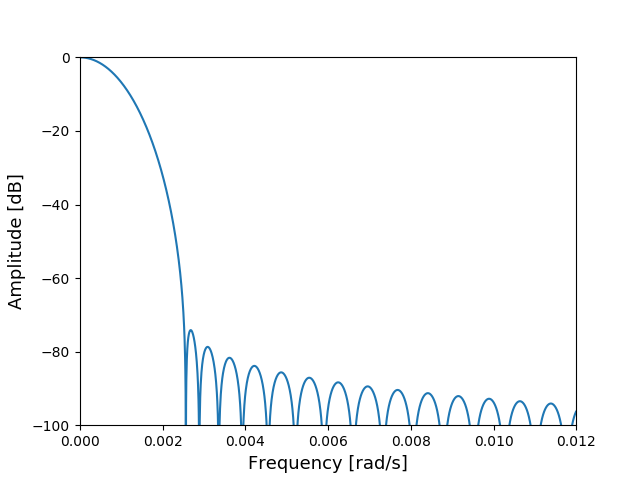
\includegraphics[width=\textwidth]{figures/dbplots/stft_bilag/8192/kaiser10.png}
\caption{Kaiser, $\beta=10$}
\end{subfigure}

\caption{Amplitude response of window functions of order $M=8192$}
\label{fig:db_plots_8192}
\end{figure}




\clearpage